\documentclass[a4paper,10pt]{scrreprt}
\usepackage[top=2cm,bottom=2cm,left=2cm,right=2cm]{geometry}
\usepackage[utf8]{inputenc}
\usepackage{graphicx}
\usepackage[german]{babel}
%opening

\usepackage{fancyhdr}
\usepackage{pdfpages}
\renewcommand{\familydefault}{\sfdefault}
\newcommand{\pic}[2][figure]{\begin{figure}[h]
 \centering
 \includegraphics[scale=0.4]{#2}
 % rsc.png: 0x0 pixel, 0dpi, 0.00x0.00 cm, bb=
 \caption{#1}
\end{figure}
}
% Code listenings
\usepackage{color}
\usepackage[T1]{fontenc}
\usepackage{xcolor}
\usepackage{listings}
\usepackage{caption}
\DeclareCaptionFont{white}{\color{white}}
\DeclareCaptionFormat{listing}{\colorbox{gray}{\parbox{\textwidth}{#1#2#3}}}
\captionsetup[lstlisting]{format=listing,labelfont=white,textfont=white}
\lstset{
 language=Java,
 basicstyle=\footnotesize\ttfamily, % Standardschrift
 numbers=left,               % Ort der Zeilennummern
 numberstyle=\tiny,          % Stil der Zeilennummern
 stepnumber=5,              % Abstand zwischen den Zeilennummern
 numbersep=5pt,              % Abstand der Nummern zum Text
 tabsize=2,                  % Groesse von Tabs
 extendedchars=true,         %
 breaklines=true,            % Zeilen werden Umgebrochen
 frame=b,         
 %commentstyle=\itshape\color{LightLime}, Was isch das? O_o
 %keywordstyle=\bfseries\color{DarkPurple}, und das O_o
 basicstyle=\footnotesize\ttfamily,
 stringstyle=\color[RGB]{42,0,255}\ttfamily, % Farbe der String
 keywordstyle=\color[RGB]{127,0,85}\ttfamily, % Farbe der Keywords
 commentstyle=\color[RGB]{63,127,95}\ttfamily, % Farbe des Kommentars
 showspaces=false,           % Leerzeichen anzeigen ?
 showtabs=false,             % Tabs anzeigen ?
 xleftmargin=17pt,
 framexleftmargin=17pt,
 framexrightmargin=5pt,
 framexbottommargin=4pt,
 showstringspaces=false      % Leerzeichen in Strings anzeigen ?        
}
\usepackage{framed}
\begin{document}
\begin{titlepage}
\title{Applikationssicherheit}
\author{Roland Hediger}
\end{titlepage}
\maketitle
\newpage

\pagestyle{fancy}
\section{App Sec Intro}
Sicherheit ist nicht nur technisch sondern politisch. Technische seite der Sicherheit, ist nicht kontroverse.\\

\subsection{Apsec Goals}
\begin{itemize}
 \item Vertraulichkeit
 \item Integrität : Modifizierungen.
 \item User Authentication
 \item User Authorization : Access control rules. 
 \item Non repudiation
 \item Verfügbarkeit
\end{itemize}
Robust - Reliable - Safe programs.

\subsection{Sicherheitsprobleme Statistisch}
55\% human error. \\
Definition : Hacker ist ehrlicher typ. Täglich hochkompetent : Besitzt Ethik
Cracker sind richtige Hacker. \\

\subsection{Sicherheits Attacken}
\begin{itemize}
 \item Interception of traffic flow : cofindentiality attack.
 \item Iterruption of service ddos attack.
 \item Modification of information : itegrity.
 \item Fabricated Info : Authentication attack.
 \item Exploit of holes : all of the above.
 
\end{itemize}

\subsubsection{Zustand des Internets}
\begin{enumerate}
 \item Wir können nicht auf intelligenten benutzer verlassen.
 \item Wir können nicht auf korrekte config von anderen verlassen.
 \item Modelle bassiert auf assertions (Zertifikaten) sind nicht zuverlässig.
 \item Nicht auf detection verlassen.
 \item Kann nicht auf ISPs verlassen.
 \item Jüristische mitteln sind nicht zuverlässig. 
\end{enumerate}

\subsection{Realistische Bemerkungen}
\begin{enumerate}
 \item Dorf und schlechte leute sind die Risiken.
 \item High tech Attacken nicht wahrscheinlich.
 \item Unerwarte Low tech Tools sind eher wahrscheinlich.
 
\end{enumerate}

\textbf{Je raffinierte der Abwehr je mehr brutal der Attacke}
       

\chapter{ssl}
\section{Verschlusselung}
\begin{description}
 \item [symetrische Verschlüsselung:]im vorraus Geheimnis vereinabren. K
\end{description}

$ k = 0111... $\\
$ A \longleftrightarrow B $\\
$ M \rightarrow e_k^{AES}(m)\\$
$ d_k^{AES} (e_k^{AES}(m)) = m $
Wir benutzen Diffie Helman um K zu vereinabren.
K ist vereinbart also ist Authentication gelöst. 

\begin{description}
 \item [asymmetrische Verschlusselung] Zwei Partner. Keine Vereinbarung
\end{description}
$ A \longleftrightarrow B$\\
$ A : PK_{A} $ und $SK_{A}$\\
$ B : PK_{B}$ und $SK_{B} \\$
$ e_k^{M} $ wo $e$ ist RSA und $k=PK_B$ \\
$ d_k(e_k^{M}) = M$ wo $d$ ist RSA und $k = SK_B$ für $d_k$\\

Satz : $n \ge 0 : n = p_1.p_2...$ \\
Vermütung : Effizienten methoden Zahl > 0 in Primfaktoren zu teilen.
Polynomial : höchtens $x^n$ Schritten.
500 - 1000 digit Zahlen.  Quantum Computer macht dieses Problem in P Zeit.

Athentication is inherent in def von RSA weil nur B kennt dass usw.

\section{Bedeutung von Integrität}
$ A \longleftrightarrow B $
M muss guarantiert nicht unterwegs manipuliert worden.
Oscar muss kein Zugriff haben. Meldung im Klartext geschickt.
$ A : sha3(m) = t, m,$  t geschickt, B macht $sha3(m) = t1, t==t1?$\\
Es gibt aber ein Sicherheitsfehler. \\
Was kann Oscar machen? \\
$ m'' ,t'' \longleftrightarrow B $  Man in the middle. \\\
\textbf{Methode um hash weniger manipulierbar zu machen -} Digitale Signatur \\

\subsection{Digitale Signatur}
\textbf{RSA Signierung:}
$A \longleftrightarrow B$ \\
$M,e_{k=SK_A}(h^{SHA3}(m))$ wird geschickt wo e ist RSA.\\
$B(e_{k=SK_A}(h^{SHA3}(m)))$ B macht $t' = sha3(m)$ und $d^{RSA}_k(e_{k=SK_A}(h^{SHA3}(m))) = sha3(m)= t1'$\\
$ t1' == t'?$ \\
Teil von SSL, aber beweisbar sicher? Oscar Attackenmöglichkeit : B arbeitet mit $PK_A$ Oscar kann es auch tun.\\

$ e_k=SK_A (sha3(m))$ \\
$ d_k=PK_A (e_k(h(m))) \rightarrow h(m)$ \\ message inertcept and then can get m because using PKA
oder :
MAN IN THE MIDDLE $SK_{OSCAR}$ SIGNIEREN und falschen. \\

\section{Real secure Channel}
\pic[Wirklicher Sicherer Kanal]{rsc.png}

Vereinfachte Struktur Schichten im OSI Model.\\
Uns interessieren IP / TCP Network Layer.\\
\textbf{Methoden:}
\begin{description}
 \item [IP Security] Arbeit auf Network Level - IPSEC in IP Layer. Funktioniert noch nicht so gut.
 \item [SSL] Zusätzliche schicht zwischen TCP IP und Applikation
 \item [Kerberos] Applikations Layer, schwierigste - Kerberos übernimmt die ganze Arbeit. Andere Beispiele :
 S/MIME PGP und SET.
\end{description}

Funktionsweise für TCP IP. Komm mit App. Tcp hat ein Port definiert, Port ist gebunden mit Applikation. Im Vergleich hat 
IP Source und Destination info zu schauen wehr Packet geschikt hat. \textbf{Info von unteren Layer ist im Klartext 
verfügbar.}

Applikation muss SSL Fähig sein.

\section{SSL Characteristics}
\begin{itemize}
 \item Server Public Key Authentifiziert
 \item ..
\end{itemize}

\pic[SSL Funktionalität]{sslfunc.png}

\subsection{SSL Protokoll Teilen}
\pic[SSL Teile I]{ssl_parts1.png}

Tcp Verbindungsaufbau : 
\begin{itemize}
 \item TCP Packet SYN(C) FLAG auf 1 gesetzt von a - b kein data.
 \item B empfängt Paket, schickt wiederum ein Paket SYN und AKNOWLEDGE FLAG auf 1.
 \item A schickt züruck mit AKNOWLEDGE = 1. Ab jetzt Verbindung zwischen A und B. Noch nicht vertraulich
\end{itemize}



\begin{description}

\item [Hand Shake] \textit{Einfache Version} Server gibt public key to client - Man in the middle. Schwachstelle.
\begin{verbatim}
Client : Hello, here is a list of cipher suites I can use.
Server: Hello, here is the cipher suite I chose from your list. And
here's an X.509v3 certificate that contains my public RSA
key.
Client : [Scrutinises the certificate, checks to make sure it's signed
by a known certificate authority.] Okay, thanks. Here's the
pre-master secret, encrypted with your public key. The next
thing I say to you will be encrypted with the session key.
Client : [Encrypted] I'm done with the handshake.
Server: [Decrypts the pre-master secret using private key, then
generates the session key.] The next thing I send will be
encrypted.
Server: [Encrypted] I'm done with the handshake too.
        \end{verbatim}

 \begin{enumerate}
  \item Step 3 : [] = optional. Client untersucht die gute des Zertifikats. 
  \subitem $ A \longleftrightarrow B$ (TCP IP Kanal)
  \subitem Zertifikat : $PK_{SERVER}$ drin und signiert (VeriSign)
  \subitem Problem effizienz -- PK einfach geliefert. Zertifikat hat Firmen Root Signatur.
  \subitem Client \textit{kann} prüfen. Fehlerquelle. Kontakt mit Firma aufnehmen und Prüfen. Was aber nicht wissen : 
Wer hat daten von Verisign Server.
 \end{enumerate}

 \item [Change Cipher Spec] Wechsel von Cipher Spec zur Laufzeit
 \item [Alert Protocol] Protokoll bei mögliche Attacke für Benachrichtigung
 \item [Encrypted Application Data] Selbsterklärend
\end{description}


Unten liegt Record Layer Protocol. Guarantieen Festlegen in diesem Layer, Auth Enrypt usw.

SSL ist normallerweise Protokoll unabhängig aber ist nur in der Praxis über HTTP

\pic[SSL Teile II]{ssl_parts2.png}

\section{SSL Zertifikaten}

Ein SSL Zertifikat besteht aus 3 Teilen :
\begin{enumerate}
 \item \begin{description}
        \item [Angaben über Besitzer] (Institution / Person)
        \item [Angaben über Provider] Vertraulicher Behörden, Echtheit versichern
       \end{description}
\item Digisign des Providers.
\item Public Key von Server
\end{enumerate}

\subsection{Client Überprüfung}
Folie 44.
DN= Distinguished Name.
\textbf{Client führt volgendes aus:}
\begin{itemize}
 \item Verfalldatum prüfen.
 \item Wer ist die ID die die Zertifikat verifiziert. Identifizierung von Provider : Liste von vertrauenswürdige 
Behörden (Im Browser).
 \item Wenn wahr? Sucht PK von Provider und prüft Signatur von Zerifikat. RSA Hash Wert Signatur Prüfung. Algorithmus 
für Hash im Zertifikat.
 \item \textit{Man soll} anhand von Verifizierungsprogram und von Server des Providers nochmal verifizieren.
\end{itemize}

\subsection{Nachher : Erzeugung von Session Key}
Client $ \longleftrightarrow $ Server\\
Client schickt : $ e_{k=pk}^{RSA}(Pre Master key)$ \\
Server entschlüsselt pre master key aus RSA.
Client $ \longleftrightarrow $ Server\\
Server schickt $e_{k=pre maser key}^{AES}(random_0)$ \\
Client und Server bidirectional mit $ SK = pre_master_key ++ random_0 ++ timestamp $ wo $SK =$ session key.\\
$e_{SK}^{AES} (m)$ wo m=nachricht. \\

Warum muss der Server ein Session Key machen? Schlüssen vereinbaren : Teil von Partei 1 Teil von Partei 2.\\
Sonnst Attacke : Wenn Server unter kontrolle, alles im Griff von Oskar. \\

Ein Timestamp ist zum \textbf{Replay Attack} zu verhindern : Oscar kann vorübergehend Verbindung unterbinden und bei 
Wiederaufbau verkaufen als Server.
\textit{Begrenztes Fenster}.

\subsection{Handshake im Detail}
Folie 17.
Wichtige Punkte :
\begin{itemize}
 \item Braucht funktionierende TCP/IP Verbindung.
 \item Session Key während der Sitzung ändern.
\end{itemize}

\subsubsection{Wie kann ich die Session Abschliessen?}
Tcp Header hat FIN (Finish Flag).
Alert Close warning und hash Value von allen Byte die ich bisjetzt geschikt haben und Kontrolle. und nacher kommt FIN.

\subsection{Master Secret Generierung}
Folie 20.

\section{SSL Record Protocol}
Folie 24.
Folie 27.
zufallszahlen sind wichtig.

\subsection{Bemerkung}
Optionale überprüfung. + Nur Server muss sich authentifizieren. Grösste Schwachstelle SSL.

\chapter{SSL + Java}
\section{Socket Intro}
Folie 33
Folie 37:
SSL Context. Alles abgeleitet davon. Nicht direkt im Java implementiert. Abstrakt klassen und API nicht Konkret. Sun hat 
referenz Implementation JSSE.
NIE nutzen. 

Folie 39 gut grun, rot, ist schlecht.
Aes is beste schnellste sym Verschlüsseln.


Empfehlenswert ist ``BouncyCastle'' 100\% Kompatibel.


\section{Certification path}
Folie 45. CLient macht Prüfung Lokal.
Globale Prüfung? --
Zertifikat chaining von Root zu Root Zertifikat. Verdammt langsam.


\chapter{Validation}

\section{Salzer-Schröder rules}
\begin{description}
 \item [Least privilege] Nutzer und Applikationen sollen nur minimale Persmissionen haben um laufen zu können.
 \item [Economy of mechanisms/Einfachkeit] Techniken wie Zeile pro Zeile Software zu untersuchen, sowie auch eine 
physikalische Untersuchung von Hardware sind notwendig. Für den Erfolg von sollche Techniken, ist ein kleines und 
einfaches Design essenzial.
 \item [Offene Design] Der Schutzmechanismus muss sich nicht auf die Dummheit der Angreifer verlasen. Sicherheit durch 
(obfuscation) ist blöd und gefährlich.
 \item [Komplette Verhandelung/Mediation] Jede Zugriffsversuch soll überprüft werden.
 \item [Fail Safe Defaults] Defaultmässig zugriff verweigern. Der Schutzmechanismus sollte klar die Bedingungen für 
Zugriff identifizieren können.
 \item [Teilung von Permissionen / Separation of Priviledge] Zugriff auf Objekten sollen von mehrere Bedingungen 
abhängen sodass falls ein Schicht durchgebrochen ist, keinen kompletten Zugriff geleistet werden kann.
 \item [Least common set of Mechanism] Der Betrag und die Nutzung von gemeinsamen Mechanismen minimieren.
 \item [Ease of Use] Falls Schutzen nicht intuitiv und leicht zu lernen ist, werden Benutzer es ignorieren.
 
\end{description}

\pic[Salzer-Schröder Rules]{ss-sw.png}
\pic[Web Applikation Sicherheit]{was.png}

\section{Motivation : Angriffe}
%\pic[Attacken]{attacks.png}

\subsection{SQL Injection}
Alle Webapplikationen benutzen eine Datenbank um im Backend Daten abzuspeichern.Benuztern greiffen indirekt auf der 
Datenbank zu.
\begin{itemize}
 \item Eingabe mit Webforms.
 \subitem Servlet/Script emfängt Daten
 \subitem Script benutzt SQL Query, und erzeugt Seite mit Resultaten.
 \item Kann mittels POST oder GET ausgeführt werden
\end{itemize}

\subsubsection{Login Attack}
Ocar loggt sich ein und versucht die Query so zu manipulieren dass es immer eine Zeile als Ruckgabewert hat.Mit logins 
funktioniert es oft mittels 'or' '='\\
\begin{verbatim}
 GET /path/login.pl?user='or''=' &pwd='or''=' HTTP/1.0
\end{verbatim}
Daraus folgt das diese Query immer True zurück gibt im Where Klausel, und deshalb wird nur ``SELECT * FROM USERS'' 
betrachtet.

\subsubsection{Tricks 1}
\begin{verbatim}
 GET /path/showcars.pl?brand_id=17 UNION SELECT user,pwd,1 from Users
\end{verbatim}

\subsubsection{Fazit}
Sql Injection ist mäcjtig aber nicht so leicht um auzuführen :
\begin{itemize}
 \item Applikation mit Sicherheitslüke finden.
 \item Interne DB Struktur ist der Angreifer unbekannt.
 \item Datenbank Typ ist meistens unbekannt.
 \item Gute SQL Kenntnisse von verschiedenen Produkten vorrausgesetzt.
 \item Eingespritzte SQL Queries müssen syntaktisch korrekt sein.
\end{itemize}
Strategy gebe eine Gänzefusschen ein (Hochkomma) ein um zu sehen was für ein Fehler generiert wird.

\subsubsection{Abwehr}
\begin{itemize}
 \item  validierien, eingrenzen und sanieren alle Benutzerdaten.
 \item Benutze Client Parameter nie direkt innerhalb SQl Queries.
 \item Parameterisierte Storedprocedures sind auch eine möglichkeit.
 \item Keine DB Fehlermeldungen an den Client.
 \item DB Zugriff mit minimale Permissionen.
\end{itemize}

Prepared Statement:
\begin{lstlisting}[caption=Sql Injection Prepared Statement]
 String updatestring = "update" + dbName + ".COFFEES " + "set SALES =? where COF_NAME = ?"
 updateSales = con.prepareStatement(updateString);
\end{lstlisting}

Du musst alle werte für ? angeben, es gibt SetterMethoden in der PreparedStatement Klasse. 
\begin{lstlisting}[caption=sql Injection Prepared Statement Placeholder]
 updateSalessetInt(1,e.getValue().intValue()) //validated
 pdateSales.setString(2,e.getKey()); //validated
\end{lstlisting}

\subsection{XSS Cross Site Scripting}
Information die von dem Benutzer eingegeben ist, ist oft an dem Benutzer wieder zurückgegeben.
XSS : Javascript in Webformfeld eingeben. Im Resultat wird der Script dan ausgeführt. Attacke ist auf andere Anwender 
gezielt.
Möglichkeiten für Oscar :
\begin{itemize}
 \item Beliebige js von Server hohlen
 \item Session zugriff (Session ID)
 \item Dynamisch Inhalt anpasse, Jquery.
\end{itemize}

Die Schwierigkeit ist das der Benutzer die Javascript an der Server senden muss. Sich selbst auch attakieren.
\pic[xss Beispiel]{xss1.png}
\pic[xss Beispiel]{xss2.png}

\subsubsection{Session Hijacking}
www.sillyshop.com verkauft was und speichert session-id in ein Cookie inherhalb der Browser.\\
Der Angreifer hat eine Lücke im Script gefunden.\\
Der Opfer ist eine regelmässiger Kunde.\\
Opfer hat gültige Session ID cookie von letzten login.\\
Angreifer will diese Session ID haben um sachen als Opfer zu kaufen.\\
Angriefer hat capture.php auf eigenen Server\\

\pic[Session Hijacking]{session_hijack.png}

\subsubsection{XSS Defenses}
\pic[XSS Defenses]{xss_def.png}
  

\section{Regex}

\begin{tabular}{|l|l|}
 \hline 
 \textbf{Character Sequenz} & \textbf{Auswirkung / Kommentar} \\ \hline
 woodchuck & sucht für woodchuck \\ \hline
 \slash & escape char \\ \hline
 \slash\slash & sucht für slash \\ \hline
 \slash x41 & sucht für Charakter basiert auf hex Wert. \\ \hline
 \slash t & tab \\ \hline
 \slash n & new line \\ \hline
 \slash f & form feed \\ \hline
 
\end{tabular}

Charakter Gruppierungen :
\begin{tabular}{|l|l|}
 \hline 
 \textbf{Character Sequenz} & \textbf{Auswirkung / Kommentar} \\ \hline
   [] & Undefined Char Klasse \\ \hline
   [wW]ood & How much wood does a woodchuck chuck? \\ \hline
   [abcd]* & you are a good programmer \\ \hline
   [a-zA-Z]* & beliebige Zeichenfolge aus a,z \\ \hline
   [\^(etwas)] & heisst dan nicht etwas \\ \hline
   . &  beliebige Charakter \\ \hline
   \slash d & Digit (0-9) \\ \hline
   \slash D & Non Digit ([\^0-9]) \\ \hline
   \slash s & whitespace \\ \hline
   \slash S & non whitespace \\ \hline 
   \slash w & word - zeichen + zahlen \\ \hline
   \slash W & nicht word. \\ \hline
\end{tabular}

Greedy Characters :
\begin{description}
 \item [?] Vorherige Charakter Optionale
 \item [*] 0 bis mehrere vorkommen von vorheriger Charakter.
 \item [+] 1 bis mehrere vorkommen von vorheriger Charakter.
 \item [.] Beliebige Charakter bei position von punkt. p.nt = pant punt etc.
 
\end{description}

Matching Typen:
\begin{description}
 \item [Greedy Matching] längste Match.
 \item [Reluctant Matching] kurzeste Match.
 \item [Possesive Matching] Nur längste Match auch wenn kurzere existieren.
 
\end{description}

Logische Operatoren:
\begin{description}
 \item [AND] zwei Charakter zusammen
 \item [OR] |
 \item [Grouping] () Bsp : (gupp(y|ies) = he is guppy oder guppy guppies usw.
 \item [\slash zahl] Referenziert vorhergegebenes Matching
  
\end{description}

Boundary Matchings :
\begin{description}
 \item [kappe] Zeilienanfang.
 \item [\$] Zeilenende.
 \item [\slash b] Wortgrenze
 \item [\slash B] Nicht Wortgrenze
 \item [\slash A] Input-anfang.
 \item [\slash G] Ende von vorherigem Match.
 \item [\slash Z] End of input except for final terminator.
 \item [\slash z] End of input.
\end{description}

Operator Riehenfolge:
\begin{enumerate}
 \item ()
 \item *  + ? {}
 \item Sequenzen
 \item | :
\end{enumerate}

\subsection{Java Biespiel von Regex}
\pic[Java regex I]{jreg1.png}
\pic[Java regex II]{java_regex2.png}
\pic[Java regex III]{java_regex3.png}



\chapter{Robust Programming}
\pic{cardinals.png}

For 5 system’s (SW) components of an e-commerce application in series
(e.g. the input of component i depends on the output of component (i-1)),
each of which has 98\% uptime, you should expect to be down in a one
year period 3.9 hours per day. This means, that your application without
any apparent security hole, behaves as one which is befallen by a DoS-
attack.

\section{Zuverlässigkeit in der Praxis}

Wartezeiten im Spital:
\begin{enumerate}
\item  Anruf bis Ankunft von Sanitär: 3 m
\item Warterzeit für dringende Materialen innerhalb 3 Schichten: 24 h
\item Warterzeit normalle Untersuchung: 1 \slash 4 3 weeks
\item  Ratio Routine/Notfall 1 \slash 4 10000-zu-1
\end{enumerate}
Compare with the digital world:
\begin{enumerate}
\item Dauer tragische Penetrationsangriff: 700 ms
\item Komplette wiederhohlung: 2 h
\item  Ratio rebuild/lose 1 \slash 4 10000-zu-1 
Gesundheit(Sicherheit) und Kosten sind ungefähr invers Proportional (Adi Shamir).
\end{enumerate}

99 Prozenten:\\
\begin{enumerate}
\item Six nines (99.9999\%): Mature manufacturing quality assurance
\item Five nines (99.999\%): Public switched telephone network availability (it
took 100 years to get there).
\item  Four nines (99.99\%): Domestic electrical grid reliability
\item  Three nines (99.9\%): Maximum possible desktop uptime after downtime
required by monthly patching drills.
\item Two nines (99\%): Credit card number protection (Basis: 640 m issued vs.
112205775 reported exposed in 2007 and assuming 5% of exposed cards
actually used by fraudsters).
\item  One nine (90\%): Share of Internet backbone traffic that is not broadly
related to malicious attacks.
\item  Zero nines (10\%): Aggregate ability of commercial antivirus programs to
find new malware
\end{enumerate}

\section{Java hinter der Kulisse}
\pic{javakul.png}

\section{Robustheitsregeln}

Fehlerquellen: \\
\begin{enumerate}
\item Syntax (erledigt mit gutem Kompiler)
\item Semantik (Gehirne nicht perfekte Programmierer)
\item IO oder externe Resourcen schlagen fehl. (Exception Behandelung)
\item Mehrdeutige Spezifikationen oder implementationen machen Programme kaputt. (JMM + Concurrency)
\end{enumerate}

\begin{framed}
 Gute Definition von Robustheit : Graceful behaviour in presence of errors
This means that if the program fails, it falls into a well known state and at
least logs why it has failed.
Deutsch : Ansprechende / Elegante / Gute Verhaltung falls Fehler auftreten.
\end{framed}

Möglichkeite um für Robustheit zu Prüfen : \\
\begin{enumerate}
 \item Types (Typ Sicherheit)
 \item Tests
 \item Formal Proofs (Mathematische Beweise)
\end{enumerate}


\section{Techniken für Robustheit}
\begin{enumerate}
 \item Sinnvolle benutzung von Typen und Attributen.
 \item Annotationen (Compilezeit)
 \item Exceptionbehandelung (Laufzeit)
 \item Assertions (Laufzeit)
\end{enumerate}

\section{Typen und Sichtbarkeit in Java}
\begin{itemize}
 \item Alle felder mussen private sein.
 \item Felder die Initialisiert sind vom Contructor sind nachher niemals aktualisiert/verändert.
 \item Schlussendlich Immutable. 
\end{itemize}

\begin{framed}
 The class is not immutable because a reference to a mutable field is returned.
Important: in Java, if a field (variable, parameter) is final, it does not mean that it
cannot change, only that the reference to it cannot change.
\end{framed}
\pic[Gestohlene Werte von Immutable Student Klasse]{gestst.png}
\textbf{Best Practices Immutable} 
\begin{itemize}
\item All non-private fields have to be declared final and have to be of
primitive or immutable type
\item No setter methods
\item Methods must not change the (visible) state of the object
\item Class has to be declared final (or not extensible with factory
creators’ methods)
\item Do not inherit from a base class which has non-static mutable fields
\item References returned by getter methods have to be of primitive or of
immutable type or have to be (deeply) cloned
\item References passed to the object with a constructor have to be of
primitive or immutable type or have to be (deeply) cloned
\item The this reference is not allowed to escape during construction
\end{itemize}

\section{Inheritance}
\pic{scsh.png}
 Against code inheritance:
\begin{itemize}

\item Strong relationship between base and derived class;
\item  The extension of a class with sub classing, requires an in-depth
\item knowledge about the implementation of the base class. E.g.:
\subitem  Which virtual methods are called in the base-class method?
\subitem In which state is the base-class upon invocation of virtual methods?\footnote{todo}
\item  Specialization interface means:
\subitem Protected methods: Disrupts the private/public only model.
\subitem Specialization semantics
\item Inheritance breaks encapsulation:
\subitem Support for inheritance implies that (some) implementation details have
to be published!
\end{itemize}

\subsection{Using composition instead}
\begin{framed}
 To use composition in Java, you use instance variables of one object to
hold references to other objects. If call-backs are needed then this can be provided through
delegation i.e.: through explicit passing of the
reference. Alternatively you can implements a call-back
interface.
\begin{description}
 \item [+] Only Interface
 \item [+] No callbacks. 
 \item [+] No dependency on the implementation.
\end{description}

\end{framed}

 \subsection{Template Hooks}
 \pic{thooks.png}

\section{Annotations}
Annotations provide data about a program that is not part of the program
itself. They have no direct effect on the operation of the code they
annotate.

\begin{enumerate}
 \item Information for the compiler : Annotations can be used by the
compiler to detect errors or suppress warnings.
\item  Compiler-time and deployment-time processing : Software
tools can process annotation information to generate code, XML
files, and so forth.
\item Runtime processing : Some annotations are available to be
examined at runtime
\item Annotations act mostly at compile-time: and this is a very good thing. We want
to catch all of our subtle and not so subtle errors at compile time and not at run-
time in front of an important customer ...
\item Annotations can be extracted by external tools. Instead of looking for methods
with a particular name or signature, retrieve all methods with a specific
annotation.
\item Annotations are like classes. They have a specific type. They can contain fields
to store details.
\item Meta-specifications for annotations include:
a) Where they can appear on (e.g. only on classes, or only on methods)
b) A retention policy: when and where they are made available:
\end{enumerate}

\subsection{Meta Annotations}
\begin{description}
 \item [@Target] Defines to which elements an annotation might be applied, ElementType.Field, ElementType.Methode
 \item [@Retention] Specifies whether the annotation is only available for: Source (Compile, disgarded),class : class 
file storage, disgarded vm, or 	runtime, all retained, accessible using reflection
\item [@Inherited] The annotation get applied to subclasses as well (only class
annotation)
\item [@Documented] Appears in Javadoc.
\item [Examples > 1.6] \begin{itemize}
                  \item Deprecated : runtime, 
                  \item SurpressWarnings : source,
                  \item override : source
                  \item Immutable : marker interface
                  \item Annotation with Value : \begin{verbatim}
                                                  @interface Todo . {
                                                  String value
                                                  }
                                                \end{verbatim}	
                  \item Annotation with Parameters : \begin{verbatim}
                                                      @Authors {String[] names} -- @..(names=)
                                                     \end{verbatim} 


                 \end{itemize}
\item[@Resource] \pic{resc.png}
\item [@PostConstruct, @preDestroy] \pic{pcnst.png}
\end{description}

\subsection{Override Annotation}
\begin{itemize}
 \item Removal of a method in a base class:
\item overwriting methods (@Override) are flagged by the compiler
\item  Signature change of a method in a base class:
\item  overwriting methods (@Override) are flagged by the compiler
\item  Introduction of a new method in base class:
\item  A method with the same name/signature may already exist!
\item Would only be detected if
would be mandatory
\item Eclipse allows to set a flag to issue warnings if overwriting methods are
not declared as
\item  Since Java6: can also be applied on methods which implement interface
methods
\end{itemize}

\subsection{CheckReturnValue annotation}
 Suspicion that a method changes an object rather than returning a new object.\\
For example, consider the trim method in java.lang.string . This method creates a new String that is the same as the 
old 
String except thatwhite space has been removed from each end. The original String is not
changed at all, nor is anything else. Thus if one invokes it like so:s.trim();
absolutely nothing happens:\\

The correct way to invoke it is by assigning the result to a variable, possibly the same one that was used to invoke 
it: 
s = s.trim();\\
Failing to do this is a very common mistake and a frequent source of hard-to-
find bugs. By placing the annotation on a method, we tell the compiler that it should issue a warning if the return 
value isn't used.

\subsection{Null Checking Annotations}
\begin{description}
 \item [@NonNull] The annotated element must not be null. Annotated fields must not be null
after construction has completed. Annotated methods must have non-null
return values.
 \item [@CheckforNull] The annotated element might be null, and uses of the element should check
for null. When this annotation is applied to a method it applies to the method
return value.
\end{description}

\pic{cnex.png}
\pic{cnpr.png}
\pic{cnsl.png}
\subsection{@Inherited Annotation}
y default annotations are not inherited. If an annotation type has the
meta-annotation @Inherited
then an annotation of that type on a class will cause the annotation to be inherited by sub-classes.@Inherited
annotations are not inherited when used to annotate anything other than a
type. A type that implements one or more interfaces never inherits any
annotations from the interfaces it implements. Example:

\begin{lstlisting}[caption=Inherited Example Annotations]
 @Target(Element.Type)
 @RetentionPolicy(RetentionPolicy.RUNTIME)
 @Inherited
 public @interface CarAnnotation {...}
\end{lstlisting}

\pic[Inheritance Test Annotations]{inhanno.png}

\subsection{Java Type Checking}
\pic[Java Typechecking]{typechecker.png}

\subsection{Tainted and Untainted Data}
\begin{lstlisting}[caption=Tainted and Untainted Annotations]
protected void doGet(@Tainted HttpServletRequest, request,@Untainted HttpServletResponse response) throws 
IOException,servletException{
}
\end{lstlisting}

These annotations define precisely the contract in web applications. For
example data from the outside are always @Tainted ; data from the inside
(constant strings) are @Untainted and data that have been sanitized are
marked as @Detainted . Data annotated with @Tainted must always not only be validated but also specially processed to 
hinder cross-script
attacks.
\section{Custom Annotations}

Annotations need tools to process them too.
Sample Listener : 
\begin{verbatim}
 @ActionListenerFor(source="MyButton) void doSomething(){}
 \end{verbatim}

\begin{lstlisting}[caption=Custom Listener Steps]
 //STEP 1
 @Target(ElementType.METHOD)
 @Retention(RetentionPolicy.Runtime)
 public @interface ActionListenerFor{
  String source.
 }
 
 //Example with tool processing.
 
 public class ButtonFrame extends JFrame {
 public ButtonFrame(){
  panel = new JPanel();
  add(panel);
  panel.add(yellowButton);
  ToolForActionListenerFor,processnnotations(this);
 }
 @ActionListenerFor (source=yellowButton)
 public void yellowBackground(){
  panel.setBackground(Color.Yellow);}
  
 }
 //usw für Bluebutton..
 
 //ANNOTATION TOOL
 public class ToolForActionListenerFor{
 
 public static void processAnnotations(Object obj) {
  try{
  Class<?> cl = obj.getClass();
  for (Method m : cl.getDeclaredMethods()) {
   ActionListenerFor a = m.getAnnotation(ActionListenerFor.class);
   if (a != null) {
    field f = cl.getDeclaredField(a.source);
    f.setAccessible(true);
    addListener(f.get(obj),obj,m);
    }
   }
  }
  }catch (Exception e) {
  }
  }
 }
 }
 }
 
 //step 3 AddListener
 public static void addListener(Objec source,final Object param, final Method m) throws 
NoSuchMethodException,IllegalAccesException,InvocationTargetException {
  Invocationhandler handler = new Invokationhandler() {
  public Object invoke(Object proxy, Method mm, Object[] args) throws Throwable {
  return m.invoke(param);
  }
  };
  Object Listener = Proxy.newProxyInstance (null, new Class[] { java.awt.event.ActionListener.class}, handler);
  Method adder = source.getClass.getMethod("addActionListener",ActionListener.class); 
  adder.invoke(source,listener);
}
 
 
\end{lstlisting}

\section{Fault Tolerance}
\pic{ftr.png}

Fault Types :
\begin{itemize}
 \item Interface Exception : illegal service request.
 \item Internal Exception : due to mailfunction of the component itsself.
 
\end{itemize}

\subsection{Requirements for exception handling}
\begin{enumerate}
\item Simplicity: Should be simple to understand and use
\item  Unobtrusiveness: Exception handling code should not obscure the
understanding of the software: (1) and (2) are crucial for designing
reliable systems!
\item  Efficiency: Run-time overheads should be incurred only when handling
an exception. This may be relaxed, e.g. if speed of recovery is not
critical
\item  Uniformity: Uniform treatment of exceptions detected both by the
environment and by the program
\item  Recovery: It should allow recovery actions 
\end{enumerate}

\subsection{Exception Classification}
\begin{description}
 \item [Who detects the error?] \hfill \\
 Environment,Application error detection.
 \item[When is it detected?] \hfill \\
 \textbf{Synchronously:} as an immediate result of a process attemting an inappropriate operation.\\
 \textbf{Asynchronously:} some time after the operatio ncausing the error. May be raised either in the process which 
excecuted the operation or in another process. The latter is also calld asynchronous notification or signal. Mostly an 
issue with concurrent programming.
\item[Examples] \begin{enumerate}
                 \item Array out of bounds error, divide by zero. Raised Synchronously, detected by the environment.
                 \item Assertion failiure : Application detected, raised synchronously.
                 \item Failiure of monitoring mechanism (interrupt, timeouts) : Detected by the environment and raised 
asynchronously.
\item Error condition occured earlier  in another process , aside from the running one. Detected by application and 
raised asynchronously.
                \end{enumerate}

\end{description}

\subsection{Exception handling}
\begin{description}
 \item [Possible Actions:] \begin{itemize}
                            \item Ignore Exception : always bad
                            \item Error message : program continues on.
                            \item Request new data.
                            \item Retry (limited by timeout or number of tries)
                           \end{itemize}
\item [Responses to said action failing:] \begin{itemize}
                                           \item Exit
                                           \item Exit and log,
                                           \item Throw a new Exception
                                          \end{itemize}

\end{description}

\subsection{Exception handling in Java}
From the Java documentation: An Error
is a subclass of Throwable
that indicates serious problems that a reasonable application should not try to catch. Most such errors are
abnormal conditions. A method is not required to declare in its throws clause any
subclasses of Error that might be thrown during the execution of the method but not
caught, since these errors are abnormal conditions that should never occur.

Must catch all Exceptions including the ones that are not checked : UncaughtExceptionhandler.

\pic{uex1.png}
\pic{uex2.png}
\pic{uex3.png}
\pic{uex4.png}

\subsection{Assertions}
\begin{description}
 \item [Pre Condition] A condition that the caller of an operation agrees to satisfy.
 \item [Post Condition] Callee itsself satisfies condition.
 \item [Invariant] satisfied anytime a client invoks any of its object's methods a condition that should always be true 
for a segment of a program.
\end{description}

Can be enforced with java assertions.
\pic{aex1.png}
\pic{aex2.png}
\pic{aex3.png}

\pic[Enabling Assertions]{aex4.png}

\chapter{Access Control}
\pic{acc.png}

\begin{description}
 \item [Authentication] enables/verifies the identity of Requester. Requester presents credentials 
(knows/possesses/is--biometric). 
\item [Authorization] Does he have the right to perform certain actions?
\item [Auditing] process gathers data to discover violations or diagnose their cause. \textit{Offline or after the fact}
\end{description}

\section{AC Policies + Mechanisms}
Subjects (e.g. users, agents) detain privileges (e.g. rwx) on objects (e.g. data, programs, devices) according to AC 
policies (models).
\begin{description}
 \item [Policy] Specifies how accesses are controlled and access decisions are determined. 
 \begin{description}
  \item [Discretionary AC\footnote{AC = Access Control}] Nach Ermessen.
  \item [Mandatory AC] Verbindliche Zugriffskontrolle. 
  \item [Role Based AC] Rollenbasierte Zugriffscontrolle. 
  
 \end{description}
\item [Mechanism(Structure)] implements or enforces policy. 
\begin{itemize}
 \item Access Matrix
 \item AC List (ACL)
 \item Capability List
\end{itemize}
\end{description}

\section{Discretionary AC}
This policy restricts access to the system based on the identity of users, and or the groups to which they belong.
Examples are in *nix systems where we have user / group / other. Processes can also obtain temporary permissions with 
setuid.

\begin{description}
 \item [Closed DAC] authorization must be explicitly specified. since the default decision is always deny.
 \item [Open DAC] Always access, denials specified. 
 \item [Problems with DAC] \begin{itemize}
                            \item Danger of users' mistakes or neglegance. 
                            \item Disemination of Information is not controlled. User who can read data can pass it to 
other unauthorized users to read without the owner knowing it. 
                           \end{itemize}

\end{description}

\section{Mandatory AC}
\begin{framed}
 Each subject and each object is assigned a security level. 
 \begin{itemize}
  \item Subject's label / clearance specifies level of trust for object. 
  \item Objects label is required level of trust to access that object. 
 \end{itemize}

\end{framed}
\begin{description}
 \item [+] Reduction of possible damage. 
 \item [-] Loss of flexibility.
\end{description}

\section{Multilevel Security}
\textbf{Implementations:}
\begin{enumerate}
 \item Military security Policy : Classification involves sensitivity levels and compartments. Information must not 
leak into unclassified files. 
\item Group individuals and Resources : Use some form of heirarchy to organize policy. Only marketing people can have 
access to sales statistics for example. 
\item Other policy concepts include : Separation of duty and the ``Chineeese Wall Concept''
\end{enumerate}

\section{Bell-LaPadula Model}
\pic{blp.png}

Set of Subjects, and Objects O . Each subject $s \in S$ and $o \in O $ have a fixed security class $L(s)$ (clearance) 
and a classification $L(o)$ Each $s$ has a maximal and an actual security level. Security classes are ordered : \\
$TS$\footnote{Top Secret} $> S$\footnote{secret} $ > C$\footnote{classified} $ > UC$ \footnote{unclassified}

\begin{framed}
 \begin{description}
  \item [Simple Security Policy] s may read object o only if $L(o) \le L(s) $
  \item [*-property] If subject s has read access to object o then s may write into object p if $ L(o) \le L(p)$
  \item [Basic Security Theorem] Let $\Sigma$ be a system with an initial state $\delta_0$ and let T be a set of 
transformations . If every set of T preserves the above  principals then $\forall \delta_i \in \Delta i \ge 0$ is 
Secure.
 \end{description}
\end{framed}
\section{Other Policy Concepts}
\begin{description}
 \item [Separation of Duty] \begin{itemize}
                             \item – If amount is over \$10,000, check is only valid if signed by two
authorized people
\item Two people must be different
\item  Policy involves role membership and physical difference
                            \end{itemize}
\item[Chineese Wall] Lawyers L1, L2 work in the same firm
If company C1 sues C2:
\begin{itemize}
\item L1 , L2 can each work for either C1 or C2
\item  No Li can work for opposite sides in any case
\end{itemize}
Not representable in matrix.
\end{description}

\section{Role based Acess Control}
Premissions are associated with roles and users/subjects.
\begin{description}
 \item [Roles] Set of actions and responsibilites associated with particular working activities.
\end{description}

Simplifies the management of permissions because 
\begin{itemize}
 \item decisions based on roles of users within organisation.
 \item Roles have overlapping privledges and responsibilities. 
 \item Roles permissions can be updated without updating individual users. 
 \item Enterprise specific policies. 
 \item Closely related to user groups.
\end{itemize}
RBAC are hierarchies with delegation of powers
and rights.
Roles
Users
In the example on the left side a user of role doctor has
access to all transactions defined between intern and healer.
The user with role healer on the contrary is restricted to his
resources. A doctor can delegate a task to an intern or to a
healer.
RBAC allows for least privilege (Saltzmann,
Schröder) since a user with higher privileges
doesn't need to activate them until he really needs
them.
RBAC does require (i) some rules for role
assignments and authorization and for transaction
authorization and (ii) rules for delegation of
credentials. A RBAC security policy is fully
implemented in JAAS.

\pic[RBAC Example]{rbacex.png}

\section{Access control Matrix}

\begin{itemize}
 \item Describes protection state accurately between subjects and objects.
 \item Elements describe rights of subjects over objects. 
 \item State transisions change the elements of a matrix.
 \item Example : Linux Kernel : \begin{verbatim}
                                 getfactl, setfactl
                                \end{verbatim}

\end{itemize}

\pic[ACM Construction]{acmconst.png}
\pic[ACM Example]{acmex.png}
\pic[ACM Example 2]{acmex2.png}

\pic[Linux Permissions] {linp.png}

\subsection{Right to copy}
\begin{verbatim}
 r : read right that cannot be copied
 rc : read right that can be copied.
\end{verbatim}

Allows processor to give rights away.  Often attached to a right, so it only applies to that right. 
Is copy flag set when giving right r the rc right.

\subsection{Atenuation of priveledge}
This principle says you can’t give away rights you do not possess.
See point 1 of Saltzman/Schröder. \textit{Restricts rights in the system}

\begin{framed}
 This is ignored, owner gives rights to self and others and can delete. 
\end{framed}

\subsection{Summary}
\begin{itemize}
 \item ACM simplest abstraction mechanism for protection state within a system
 \item Transisions alter protection state.
 \item Six primitive operations alter the AC matrix: Transitions can be
expressed as commands composed of these operations and,
possibly, conditions.
\end{itemize}

\subsection{ACL}
\pic{aclacm.png}
\pic{cl.png}

\begin{description}
 \item [Access Control List] \begin{itemize}
                              \item Associate list with each object.
                              \item Check user/group against list.
                              \item Relies on authentication - NEEDS TO KNOW USER.
                             \end{itemize}
\item [Capabilities] Capability is an unforgeable ticket. Random bit sequence + TS protected by crypto or managed by OS.
Can be passed from one process to another. Reference monitor checks ticket. \textbf{Does not need to know or 
authenticate user/process}. Separation of privledges: Authentication and then Authorization through capability list.
\item[Delegation] \begin{itemize}
                   \item Capability : Process can pass capability at run time.
                   \item ACL : commonly let other process act under current user.
                   
                  \end{itemize}
\item[Revocation] \begin{itemize} \item ACL : Remove user or group from list.
                   \item  Capability can I get capability back from process : Possible in some systems if OS knows 
which data is associated with capability. If capability used for multiple resources one has to revoke all or none. 
		  \item capability points to pointer to resource  If $C \rightarrow P \rightarrow R,$ then revoke 
capability C by setting P=0.
                  \end{itemize}

\item [Authorization Relation] \hfill \\
\pic[Authorization Relation]{aclr.png}

\end{description}

\chapter{Android}
 
Challenges:
\begin{description}
 \item [Battery Life] Conserve Power. Save state so that they can be restarted later, helps to stop DOS attacks.Most 
foreground activity is never killed.
\item [Market] Not reviewed by Google. No way of stopping bad apps from showing up on market (community based approach)
Malware writers may be able to get code onto platform: shifts
focus from remote exploit to privilege escalation.
\end{description}


\section{Application Components}
\begin{description}
 \item [Activity] Defines the user interface:
 Example: scroll through your inbox. Email client comprises many
activities
\item[Service]  Java daemon that runs in background Example: application that streams an mp3 in background.
\item[Content Provider] Store and share data using a relational database interface.
\item[Broadcast Reciever] “mailboxes” for messages from other applications.
\item [Intent - Absicht] asynchronous messaging system
– Signal an intent to switch from one activity to another \\
– Example: email app has an inbox, a compose activity, a viewer\\
activity
- User click on inbox entry fires an intent to the viewer activity,
which then allows the user to view that email\\
\pic[Intent in Android]{aint.png}
\end{description}

\section{Application Signing}
Developers sign applications
Self-signed certificates:\\
\begin{itemize}
\item  Is not a form of identity
\item It is used to allow the developer who built the application to
post updates
\item It is based on Java key tools and jar signer
\end{itemize}

\section{Application sandbox}
\begin{itemize}

\item Each application runs with its UID (Linux process) with its own Dalvik
virtual machine:
\item Provides CPU protection, memory protection
\item  Authenticated communication protection using
Unix domain sockets:
\subitem Only zygote (spawns another process) and ping
run as root
processes
\item Applications announces permission requirement (security policy):
\subitem Create a white list model: user grants access
\subitem Inter-component communication reference monitor checks
permissions
\end{itemize}

\section{Android ACL}
\pic{anacl.png}
Two forms of security enforcement:
\begin{itemize}
\item Each application executes with its own user identity as Linux
process
\item Android middleware has a reference monitor that mediates the
establishment of inter-component communication (ICC)
First is straightforward to implement, second requires careful consideration
of mechanisms and security policy. 
\end{itemize}

\section{Policy Enforcement}
Android focuses on Inter Component Communication (ICC) whose security
policy is defined in the Android manifest file. It allows developers to specify
an high-level ACL to access the components:
\begin{enumerate}
\item Each component can be assigned an access permission label
\item Each application requests a list of permission labels (fixed at install)
\end{enumerate}
\pic{anman.png}

Each Android application has an AndroidManifest.xml
file which describes all the components it uses.\\
Components cannot execute unless they are listed. In the file we specify:
Rules for “auto-resolution”\\
Runtime dependencies\\
Optional runtime libraries\\
Access rules\\
Required system permissions\\

\begin{framed}
 The manifest file spells out the security policy of the whole application
\end{framed}

\subsection{Component Interaction}
\pic{compint.png}

\pic{amfest.png}

The components of an apllication can be public orp private. The manifest defines an \underline{exported}  attribute 
(with value true or false) It specifies whether the caticity can be launched by components of other applications. false 
= internal (same user id). \textbf{Default depends on intent filter rules.} Components may unknowingly become <ccesible 
to other apllications.
\begin{framed}
 Always specify the setting.If the manifest file does not specify an access permission on a public component,
any component in any application can access it.This is defensible when for instance some components provide “global”
access: e.g., the main Activity for an Application.Components without access permissions should be exceptional cases,
and possible inputs must be carefully analysed (consider splitting
components).
\end{framed}
\begin{framed}
 The code broadcasting an Intent can set an access permission restricting
which Broadcast Receivers can access the Intent.
Thus we specify explicitly which application can read the broadcast.
Implication: If no permission label is set on a broadcast, any unprivileged
application can read it.
Always specify an access permission on Intent broadcasts (unless you
specify the destination explicitly).
\end{framed}

\pic[Specification of Interaction Example]{speint.png}

\subsection{Content Providers}
Content providers are the standard interface that connects data in one process with code running in another process.

When you want to access data in a content provider, you use the ContentResolver object in your application's Context to 
communicate with the provider as a client. The ContentResolver object communicates with the provider object, an 
instance 
of a class that implements ContentProvider. The provider object receives data requests from clients, performs the 
requested action, and returns the results.

Content Providers have two additional security features: (i) separate “read”
and “write” access permission labels, and (ii) URI permissions to specify which
data subsets of the parent content provider permission can be granted for.
These features give more control over application data.

\begin{framed}
 Always define separate read and write permissions. Use URI
permissions to delegate rights to other components.
\end{framed}
\pic{cpp.png}

\subsection{Permission Categories for Content Provider}
\pic{permcat.png}

\chapter{Java Antipatterns}
\section{Terminology}
\pic{javtermssec.png}
\begin{description}
 \item [PAP] Policy Admin Point \texttt{java.security}
 \item [PIP] Policy Information Point \texttt{java.policy : grant codeBase 
..\{permission.java.security.Allermissions;\}}
 \item [PDP] Policy Decision Point : \hfill \\
 \begin{lstlisting}[caption=PDP]
  if (sm !=null) {
  context = sm.getSecurityContext();
  FilePermission p = new FilePermission(filename,"read");
  sm.checkPermission(p,context);
  }
 \end{lstlisting}
\item [PEP] Policy Enforcement Point : 
\texttt{SecurityManager,Permission,AccessController,AccessControllerContext,ProtectionDomain}
\end{description}

\section{Visibility Modifiers}
\underline{Interfaces and Classes:}
\begin{description}
 \item [public] open to all and sundry. All parts of the application can use it.\textbf{If no modifier is specified 
then open only within the same package} \underline{Problematic with inner classes}
\end{description}
\underline{Fields and Methods}
\begin{description}
 \item [Public] All parts of the application can use it.
 \item [Protected] Can be used only in the same package and from subclasses in other packages.
 \item [No modifier] Can be used only in the same package (default)
 \item [private] Only within the same class. 
 
\end{description}

\section{Purpose}
\begin{description}
 \item [Information Hiding] The visibility of a class (interface, field, method)
should be as restricted as possible. A good mantra: Keep all the
member variables private and let only those methods as public that are
important for the API.
\item [Compartmentalization of programs' components:]lear divide between
the things you should know (public) and the things you can safely
ignore (private).

\end{description}
\begin{framed}
 You may think that a secret may be embedded in an object in its private
field. It is not a very smart idea, but it is done often.
You may think that untrusted code can be prevented from executing
sensitive code by simply placing it in a package-local class. Here too, it is
not a very smart idea, but it is done often.
\end{framed}

\pic[Visibility Robustness Effects]{vbre.png}

\begin{framed}
 Java allows increasing (but not decreasing) the visibility of a member. The
situations where this is desirable are very rare and in any case dangerous
because in so doing, one breaks the API contract.
\end{framed}

\subsection{Why Protected and Default?}
Clean API can be achieved with public and private, so why protected and default?\\
\begin{description}
 \item [Protected?] \hfill \\
 \begin{itemize}
  \item A malicious client can have a class that claims to have the same
package;
\item A malicious client can have a class that extends a trusted class and
accesses protected fields.
\item \underline{But it would be nice to have a simple method to prohibit packages from being
added to an application. Unfortunately, Java does not offer any easy and robust
way to do this.}
 \end{itemize}

\end{description}

\section{Prevent Joining of Packages - Adding Malicious Packages}
\subsection{Sealing}
\pic[Sealed JAR Archives]{sja.png}
\subsection{Signing}
\pic{sg1.png}
\pic{sg2.png}

\section{Joining packages with PAP}
Insert into security file :  \texttt{package.definition=com.ibeco.securepackage}
This would mean that extra permissions would be needed to add a malicious class to package. \textbf{However noc lass loaders currently implement what is necessary to check this}

\section{Inner Classes}
\begin{enumerate}
 \item Classes defined as members of other
classes.
\item nner classes are allowed to access
private members of the enclosing
class and vice versa.
\item For each instance of the outer class
there is a corresponding instance of
the inner class.
\item Useful especially for defining in-line
implementations of simple interfaces.
\end{enumerate}


 Inner classes are not understood by JVM.
 Java compilers just transform inner classes into top-level classes:
\begin{itemize}
 \item  But JVM prohibits access to private members from outside
the class!
\item So the compiler provides access to private fields accessed
by inner (outer) classes via package-local methods
\end{itemize}

\pic[Inner class Example]{classex.png}

\begin{framed}
 The private data members of classes get exposed through the
access functions
Other classes belonging to the same package can call the access
functions and tamper the private data member
\end{framed}
\pic{unacin.png}

\begin{framed}
 \begin{description}
  \item [William Pough Proposal:] Only to the inner classes may access the private
members of the enclosing class.\\
A secret key is shared between all the classes that need
access to each others private data members:
\begin{itemize}
\item Class B wants to access a class A private member m
\item Class B invokes A’s access function
\item Class B passes its shared secret key to A’s access function
\item Class A verifies whether class B’s secret key and class A’s secret
key are the same object:
\subitem if yes, give access to its private variable m
\subitem otherwise, throw a security exception
\item The new implementation is built on top of the current
implementation:
\subitem only class files are rewritten
\subitem No need to change the JVM
 
\end{itemize}

 \end{description}

\end{framed}
\pic{plid.png}
\pic{plimpl.png}

\subsection{Overhead of Plough Solution}
\begin{itemize}
\item For each class allowing/needing access, one needs a single static field.
\item For each set of objects needing mutual access only one object is created.
\subitem All initializations are done in a
initializer.
\subitem  One additional argument in each
method
\subitem  Few additional instructions are executed for each access call to:
\subsubitem pass the extra argument
\subsubitem verify the secret key
\end{itemize}


\chapter{Common Java Antipatterns}
 \includepdf[pages=26-,nup=2x2]{ap.pdf}
 
\chapter{Java Security Game}
\subsection{Java Security in a Nutshell}
\pic{jsn1.png}
\pic{jsn2.png}
\begin{description}
 \item [Repeat] \begin{itemize}
                 \item Check if current method has the requested permission.
                 \item if not, throw security Exception
                 \item Next Check : \textit{Check if method has amplified privledges} If so, grant permission,consider 
calling method, (moving it up the stack.)
                \end{itemize}
\item[Until Call Stack is empty] do repeat.
\item[Final Check] Has thread inherited permission? if yes, Grant if no, throw exception.
\item [Notes] Protection Domain: Stores in a per thread variable the intersection (Å) of the static
permissions of all methods invoked since its start, and grant permission on the result of
that intersection operation.

\end{description}


\subsection{Game Description}
\pic{gd1.png}
\pic{gd2.png}
\pagebreak
\subsection{Problem Description}
Define privledges neccessary to play the game : 
\begin{itemize}
 \item Access to HW Resource Screen
 \item Hard disk access.
 \item Socket Access
\end{itemize}

Mechanism for granting access? 
\subsubsection{Code Domains}
Code Domains are based upon origin of the code (www.game.org,www.sgi.com) and the digital signature of the code. 

\subsubsection{Policy Files}
\begin{lstlisting}[caption=Java Policy Files for the Game]
 grant CodeBase "http://www.game.org-"{
 permission java.lang.RuntimePermission "Screen",
 permission java.net.Socketpermission "server.game.com";
 permission java.io.FilePermission "C:\\HighScore","read","write";
 }
 
 grant CodeBase "http://www.sgi.com/-" Signed By "SGI" {
 permission java.lang.RuntimePermission "Screen";
 permission java.io.FilePermission "c:\\lib\\3D_Data\\-","read";
 }
\end{lstlisting}

At runtime these plocies are enforced by the class \texttt{AccessController.checkPermission(..)} that automatically is 
called when the scurityManager has been activated in the shell or in main() method.

\subsection{Protection Domains}
\pic{pd1.png}

\section{Stack introspection of privledges}
\begin{lstlisting}
 boolean checkPermission (Permission toCheck) {
  Stack domainStack = getDomainStack(); // domain used for current thread
  while (!domainStack.emoty()) {
  Domain here = domainStack.pop();
  if (!here.implies(toCheck)) // no such right implies UND VON MENGEN	return false;
  return true;
  }
 }
\end{lstlisting}

\section{ACM and Stack Introspection}
\pic{inacm.png}

\section{Doprivileged - Temporary priveledge elevation}
Problem : 3D component cannot access 3d files - does not have necessary permissions. \\
Solution \textbf{Only the subject  game + 3DLib may possess this right and not the subject game alone}
Rights of subject in protection domain temporarily elevated.

\begin{lstlisting}[caption=Syntax of dopriviledged]
Object house = Accesscontroler.doPriviledged( new PriviledgedAction() {
public object run() {
 return readObjectFromDataFiles("house");
}
}

); 
\end{lstlisting}

\section{DoPriviledged StackIntrospection}
\begin{lstlisting}
 boolean checkPermission(Permission toCheck) {
 Stack domainStack = getDomainStack();
 while (!domainStack.empty()) {
 Domain here = domainStack.pop();
 if (here.IsPriviledged()){
 return true;
 }
 if (!here.implies(toCheck)) return false;
 return true;
 }
 }
\end{lstlisting}

\chapter{Byte and ClassLoader security.}
\pic{classformj.png}
\begin{description}
 \item [Byte Code Verifier] Prevent access to underlying physical machine via forged
pointers, crashes, undefined states
\begin{itemize}
 \item  Code has only valid instructions and register use
\item Code does not overflow/underflow the stack
\item Code does not convert data types illegally or forge pointers
\item Code accesses objects as correct type (as given in the constant\_pool
header)
\item Method calls use correct number and types of arguments
\item References to other classes use legal names
\end{itemize}
\item[Role of Classloader:] The loading and verification steps expel bogus class files before
they even get into the JVM. Protection domains drive all later security decisions. Namespaces keep separate classes and 
packages coming from different places.
\item[Protection Domain] Code Source + collection of Permissions.
\begin{itemize}
 \item Code Source = origin of class file (URL) + 0 or more signers (certificates)
 \item A class's protection domain is established by he class loader when the class is loaded - only the class loader 
knows the origin of the class file (url).
\item A class's protection domain is later used to make security decisions about hwat code in the class is allowed to 
do or not to do.

\end{itemize}
\item[Namespaces] The JVM considers the class ch.fhnw.bar.Bar loaded by class loader X to be differrent fron the class 
ch.fhnw.foo.Xyz loaded by the class loader Y even though the package names are the same. In other words, each class 
loader defines a seperate namespace for classes and packages. This lets same named classes and packages from differenct 
sources coexist. without having access to each others protected and packages scoped members. \textit{It also prevents 
package insertion attacks where an evil class claims to be part of a certain package in order to gain access to 
sensitive data.k}
\end{description}

\section{Java Class Loader Heirarchy}
\pic{jclh.png}
\begin{description}
 \item [User-defined class loaders vreated by the program:] The system class loader is the parent class loader by 
default. Another parent class loader can be specified explicitly. 
\item[Threads have associated context class loaders] Default Context class loader is the system class loader. A 
different context class loader can be specified by calling \texttt{Thread.setContextClassLoader()} it also has a 
corresponding getter method to obtain the actual class loader as a reference. 
\item[Delegation Model] When ashed to load a class the class loader \textbf{first asks its parent}. If the parent 
succeeds the class loader returns the class from the parent. \textbf{If the parent fails:} the class loader attempts to 
load the class itsself. The class loader is searched from \textbf{the top back down to the starting point}.
\item[Which class loader is used] You can explicitly load a class int a class loader with \texttt{loadclass()} If a 
class needs to be loaded and a class loader is not explicitly specified then the class is loaded into \textbf{same 
class loader as the code that is currently executing}
\end{description}

\section{Class Loader phases}
\subsection{Load Phase}
\pic{lp.png}
\begin{enumerate}
 \item Given the types fully qualified class name, obtain its class file as a byte sequence.
 \item Parse the class file into implementation-dependent internal data structures in the method area.
 \texttt{Possible error: first four bytes are not 0xCAFEBABE}\footnote{wtf}
 \item Resolve symbolic references to the super class.
 \texttt{Possible error: super class not accesible to this class : exception thrown}
 \item Resolve symbolic references to hte interfaces if neccessary : \texttt{Possible error : interface not accesible 
to class - exception thrown}
\item Create an instance of class Class to represent the type.
\end{enumerate}
\subsection{Verify Phase}
\pic{vp.png}
Checks a class for validity ( Byte Code verfiier) Verifies the following:
\begin{description}
 \item [Part 1]
 \begin{enumerate}
  \item Final classes are not subclassed
  \item Final methods are not overridden
  \item Every class has a super class
  \item Constant pool entries obey all specified constraints.
  \item All field and method references have valid classes,names, and type descriptors.
  \end{enumerate}
  \item[Part 2]
  \begin{enumerate}

  \item Valid intructions and register usage.
  \item Stack overflow / underflow protection
  \item Protect against conversion errors or forged pointers.
  \item Code must access objects as the correct type.
  \item Method calls must use the correct number of arguments of the corrent type.
  \item References to other classes use legal names.
  \item \textit{Goal : prefent access to underlying machine , forged pointers, crash or undefined state}
 \end{enumerate}

\end{description}

\subsection{Prepare Phase}
\pic{pp.png}
Allocates storgage for static fields- shared memory region between all classes, then sets the static values to default. 
Explicit inital values are set in init phase.

\subsection{Resolve Phase}
\begin{enumerate}
 \item Validate each symbolic class, field, and method reference. Search ineheritance heirarchy for declarations, and 
verify accessibility.
\item Replace each symbolic reference with a direct reference.
\subitem Greedy Resolution : Each symbolic rerefence can be resolved when a class is initially linked
\subitem Lazy Resoliton : Resolved later during execution when it is actually used.
\end{enumerate}

\subsection{Initialize Phase}
Execute the classes static clinit method:
\textbf{This is compiler generated and contains:}
\begin{enumerate}
 \item Code for explicit initialization of static fields. 
 \item Code from all static blocks.
 \subitem See java anti patterns for misusage.
\end{enumerate}

\chapter{Security Mechanisms in Java}
\pic{jsm.png}
\pic{jsm2.png}
\section{Java Security Algorythm}
\begin{description}
 \item [Repeat] \begin{enumerate}
                 \item Check if the current method has the requested permission if not, throw securityExcepion
                 \item Check if amplified privledges
                 \subitem Grant
                \end{enumerate}
\item[Until Call Stack Empty]
\end{description}

\section{Security Manager}
\pic{secman.png}
\subsection{Functions}
Controls :
\begin{itemize}
 \item access to files
 \item access to network resources
 \item protection of JVM
 \item System resource access
 \item Protection of Security.
\end{itemize}
Custom security manager can be used but not recommended. 
\section{Checkpermission}
Method called explicitly or implicitly as soon as the SM is activated:
\begin{itemize}
 \item Throws an exception if Permission p does not hold else returns
 \item All previous check methods are rewritten in termis of Checkpermission.
 \item Permits creation of new permissions without changing the security manager.
 \item uses the AccessController class for its functionality.
\end{itemize}
\begin{lstlisting}[caption=sample File Write Check]
 class Filewrite{
  public static void main(String[] args){
   File file = new File(...);
   try{
    file.canwrite() // calls checkPermission implicitly.
   }catch (SecurityException e){
   //print here.
   }
  }
 }
 
 Policy File:
 grant{
 permission java.io.FilePermission
 ".."//filename,"read";};
 }
\end{lstlisting}

\section{Security Policy Files in Java}
Fine grained configurable policies for both java Applet and Java applications are based on the following techniques. 
\begin{itemize}
 \item A text fiule contains the custom security policy for an application defaults : 
\texttt{java.policy,java.security} in [JRE\_HOME]/lib/security.
\item At run time one or more of the following checks are made depending on above policy:
\subitem Protectiondomain < Code Source < policy.
\subitem Java 2 Runtime Security Check algorythm 
\subitem Permission class and its sub classes
\subitem GuardedObject and guard.
\end{itemize}

\section{Structure of Policy Files}
Determines which system resources can be accessed and how they can be accessed. Becomes a java object. 
Building blocks of policy are :
\begin{enumerate}
 \item Origin and authentication of a piece of code - \texttt{Codebase}:
  \subitem An origin URL
  \subitem Set of digital signatures - any number of files in a JAR can be signed.
  \item \textbf{An entry in the policy file is specified by} \\
  \begin{verbatim}
  permission java Permission type "resource","action";
 \end{verbatim}
\item Wildcards are allowed. 
\end{enumerate}
\subsection{Example}
\pic[Java security policy file example]{jspe.png}

\section{Creating a new policy file}
 \begin{itemize}
  \item Use plicy tool or editor of your own choice
  \item Example below grants two permissions:
  \subitem to the code signed by Duke the permission to read files located in users home directory
  \subitem to Code from location \texttt{http://...} to read the file.encoding system property.
 \end{itemize}
\pic{polex.png}
\pic{polex2.png}
\pic{polex3.png}

\section{Permissions}
The permissions are positive, they grant access rather then deny access. By default nothing extra is allowed, two 
classes control these permissions, Permission and BasicPermission :
\pic{ptree.png}

Permissions have two arguments a \textbf{target} and a \textbf{Set of actions}. Applications are free to introduce new 
permission categories. 

\subsection{Permission files}
\begin{description}
 \item [Targets] file, directory, directory/file,directory/*.* directory/- (recursive), "<<ALL FILES>>".
 \item [Actions] read,write,execute,delete. Example : /tmp/-,read;
 \item [Notes] Can also have platform driven paths : \begin{verbatim}
                                                      c:\\temp\\foo
                                                     \end{verbatim}
\item[Socketpermission] \begin{itemize}
                         \item target : host specified with dns or ip adress allong with a port number or port range 
(1-5) or * or *.domain
\item Actions accept,connect,listen,resolve (resolve implied by any of the other actions)
                        \end{itemize}
 \item[Propertypermission] Target : represents access to various hava properties - java.home os.name,user.name. 
Actions: read(getProperty),write(setProperty).
\end{description}

\subsection{Basic Permission}
Base class for named permission, a permission that contains a name instead of a target-set,action pair.
Examples are ExitVM , queuePrintJob.\\
Runtime Permissions :
\begin{itemize}
 \item stopThread,modifyThread,securityManager,writeFileDescriptor,loadLibrary.[library name]
 \subitem Loadlibrary - permission to dynamic link in native libraries that are not under JVM supervision.
\end{itemize}

AWT,net and Security Permissions:\\
\begin{itemize}
 \item accessClipBoard, accessEventQueue,readDisplayPixels.
 \item Netpermissions: resetPasswordauthentication,specifiyStreamhandler
 \item Security Permissions ; 
getPolicy,setPolicy,insertProvider,addIndentityCeterficate,getSignerPrivateKey,setSighnerKeyPair.
\end{itemize}

\section{Permission Caveats}
\begin{itemize}
 \item Granting the write access to the entire file system is the same as granting AllPermission (think linux)
 \item Granting LoadLibrary permission is the same as granting everything because nobody knows ecactly in which way the 
library depends upon the systems resources. 

\section{Extra notes on the permission class}
\begin{description}
 \item [Permission Class] Encapsulates a permission granted or requested. Can be set read only - from then on it is 
immutable. Can be grouped using PermissionCollection and Permissions classes. 
\item [Jargon] Permissions granted to a ProtectionDomain : \textbf{privledges}. However no Priviledge Class exists. 
\end{description}

\section{Creating a custom Permission}
\begin{enumerate}
 \item You cannot change the built in permission types. 
 \item You can make a class that extends one of the existing permission classes like the example below:
 \item The new permissions must be referred to in the policy file:
\end{enumerate}
\begin{lstlisting}[caption=Custom Permission]
 public class WordCheckPermission extends Permission {
 public boolean implies(Permission other) {
 if (!(other instanceof WordCheckPermission)) return false;
 WordCheckPermission b = (WordCheckPermission) other;
 if (action.equals("insert")) {
 return b.action.equals("insert") && getName().indexOf(b.getName()) >= 0 ;
 }else if (action.equals("avoid")) {
 if (b.action.equals("avoid")) return b.badWordSet().containsAll(badWordSet());
 else if (b.action.equals("insert")) {
 for (String badWord : badWordSet())
 if (b.getName().inbdexOf(badWord) >= 0) return false;
 return true;
 }else return false;
 }else return false } ..}
 
 
 //Usage:
 public void insertWords(String words) {
 try {
 textArea.append (words + "\n"); 
 }catch (SecurityException e) {
 //showMessage
 }
 }
 
 class WordChextTextArea extends JTextArea {
 public boid append (String text) {
 WordCheckPermission p = new WordCheckPermission(text,"insert");
 SecurityManager manager 0 System-getSecurityManager();
 if (manager != null) {
manager.checkPermission(p);
super.append(text);
 }
 }
 }
 // Policy File
 
 grant{
 permission java.awt.AWTPermsiion "showWindowWithoutWarningBanner";
 permsiion ch.fhnw..WordChecpermission,"cocaine,ectasy,sex,gambling,booze,drugs,java","avoid";
 }
\end{lstlisting}

\section{Summary Permissions}
\begin{enumerate}
 \item The permissions of a class are calculated at load time from the policy object.
 \item But in can be delaxed until the first security check
 \item Permissions granted to classes, not objects
 \item Permissions are additive : \\
 \pic{ap.png}
 \item Only positive permissions do exist, grant never deny access. 
\end{enumerate}
\end{itemize}

\section{Protection Domains}

ProtectionDomain class :
\begin{itemize}
 \item Created form CodeSource and PermissionCollection
 \item Defines the set of permisions granted to classes, changes the PermissionCollection to change permissions.
  \item \textbf{Each class belongs to one ProtectionDomain isnstance} set at class creation time and never changed.
  \item Access to these objects is restricted, getting its reference requires \begin{verbatim}
                                                                               RuntimePermission getProtectionDomain.
                                                                              \end{verbatim}
\item One classloader can have more then one protection domain
\end{itemize}

\pic{pd.png}

\subsection{Important Classes}
\begin{description}

\item[CodeSource Class] The class extends the concept of a codebase to encapsulate URL but also certificates. This 
class is immutable.
with the abstract implies method of the permission class one can implement partial URL matches.
\begin{itemize}
 \item Permits policies to use URL patterns
 \item a.implies(b) == true means that if one is granted permission a then one would get permission b too because its 
implied..
\end{itemize}
 \item[Policy Class] It provides an interface to the user policy:
 \begin{itemize}
  \item Given a CodeSource it returns a PermissionCollection.
  \item its called during the setup stage of a Protectiondomain to set the class' permissions.
 \end{itemize}
\item[Loading procedure] \hfill \\
\pic{lp1.png}
\pic{lp2.png}
\pic{lp3.png}
\item[AccessController] Its method getContext takes a snap of current execution context ( stack trace)
\begin{itemize}
 \item The snapshot includes all ancestor threads. These contexts are stored in type AccessControlcontext.
 \item The class AccessControlcontext has a checPermission for the context it encapsulate. Results stored and used for 
limiting privledges later.
\subitem Purpose of controller : suppoer actions on behalf of another
\subitem One thread posts events to another one
\subitem Delayed actions like cron jobs
\end{itemize}

\end{description}
\pagebreak
\section{Implications of security check algorythm}
Default privledges are the intersection (Schnitt) of all class' permissions in the stacks call tree. Wthout 
doPrivleged, permissions that dcrease the privledge are permitted (Principle of least Priveledge).

doPrivileged enables all class' privleges: Like Unix setuid it enables trusted classes to use full set of privledges 
but only when requested. Without any attached context it enables all privleges this is dangerous. With context it only 
enables those privleges that are within given context. This is a safe action because the resulting privleges are always 
less then those without context.

\pic{pex1.png}
\pic{pex2.png}
\pic{pex3.png}

\subsection{Security Holes}

\begin{enumerate}
 \item If a method M1 is not overridden the protectiondomain of the supeclass is used
 \subitem The consequence of this fact is obvious: Methods running with privledges \textbf{Should not depend on 
protected variables}
\subitem A cracker could : create a subclass with method m2 that modifies variables used by m1, and causes m1 to be 
invoked with influence from m2.
\end{enumerate}

\chapter{Java Security at Method Level}
\section{Guarded Object}
\pic{go.png}
The Guarded object enapsulates its object to guard : 
\begin{itemize}
 \item asks Guard interface to determine wherger access is ok
 \item Class Permission implets Guard by calling SecurityManager.Checkpermission(self)
 \item PermissionCollection does not implement Guard.
\end{itemize}
A provider of object-to-guard does the following.
\begin{itemize}
 \item Instantiates new Guard (e.g a Permission)
 \item Instantiates GuardedObject
 \item Gives GuardedObject's reference to requestors.
\end{itemize}
Clients who wish to use object-toguard call GuardedObjects's getObject() :
\begin{itemize}
 \item CheckGuard is then called
 \item if ok ref returned else not ok then security exception.
\end{itemize}
\pic[Guarded object Usage]{gousage.png}
\end{document} 